\documentclass[t]{beamer}
\usetheme[english]{KIT}

\usepackage{amssymb} %% For \backprime
\usepackage{multicol}

%\usepackage{mathpartir}
\usepackage{graphicx}

\usepackage{tikz}
\usetikzlibrary{arrows.meta}

\usepackage[T1]{fontenc}
\usepackage{babel}
\usepackage{booktabs}
\usepackage[normalem]{ulem}
\usepackage{fontspec}
\setmonofont[Scale=MatchLowercase]{Iosevka}
%\newfontfamily\lc[Scale=MatchLowercase]{Iosevka SS09}

\usepackage{minted}
\definecolor{codebg}{rgb}{0.95,0.95,0.95}
\setminted{bgcolor=codebg,breaklines}
\usemintedstyle{tango}
\newmintinline[lean]{lean}{bgcolor=white}
\newminted{lean}{fontsize=\footnotesize}

\usepackage{newunicodechar}
\newfontfamily{\freeserif}{DejaVu Sans}
\newunicodechar{ℕ}{\freeserif{ℕ}}
\newunicodechar{ℝ}{\freeserif{ℝ}}
\newunicodechar{ₐ}{\freeserif{ₐ}}
%\newunicodechar{₁}{\freeserif{₁}}
%\newunicodechar{∈}{\freeserif{∈}}
\newunicodechar{𝓞}{\ensuremath{\mathcal{O}}}
\newunicodechar{∉}{\freeserif{∉}}
%\newunicodechar{Π}{\freeserif{Π}}
%\newunicodechar{→}{\freeserif{→}}
\newunicodechar{⦃}{\freeserif{⦃}}
\newunicodechar{⦄}{\freeserif{⦄}}
%\newunicodechar{∧}{\freeserif{∧}}
%\newunicodechar{∨}{\freeserif{∨}}
%\newunicodechar{⊢}{\freeserif{⊢}}
\newunicodechar{⊑}{\freeserif{⊑}}
\newunicodechar{ₚ}{\freeserif{ₚ}}
\newunicodechar{∘}{\freeserif{∘}}
\newunicodechar{ₗ}{\freeserif{ₗ}}
\newunicodechar{∪}{\freeserif{∪}}
\newunicodechar{𝓸}{\ensuremath{o}}
\newunicodechar{⊆}{\freeserif{⊆}}
\newunicodechar{≼}{\freeserif{≼}}
\newunicodechar{≃}{\freeserif{≃}}

\title{Towards Lean 4:\\ An Optimized Object Model for an Interactive Theorem Prover}
\author[Ullrich, de Moura]{\underline{Sebastian Ullrich}\inst{1}, Leonardo de Moura\inst{2}}
\subtitle{\insertauthor}
%\institute[IPD Snelting]{Programming paradigms group - IPD Snelting}
\institute[]{\inst{1}Karlsruhe Institute of Technology, Germany\ \ \ \inst{2}Microsoft Research, USA}
%\institute[]{\inst{1}TU Wien \inst{2}KIT \inst{3}U. of Washington
\date{2018/12/12}
\makeatletter
\sbox{\KIT@titimg}{
  \hspace{0.08\titleimagewd}
    \raisebox{0.1\titleimageht}{
      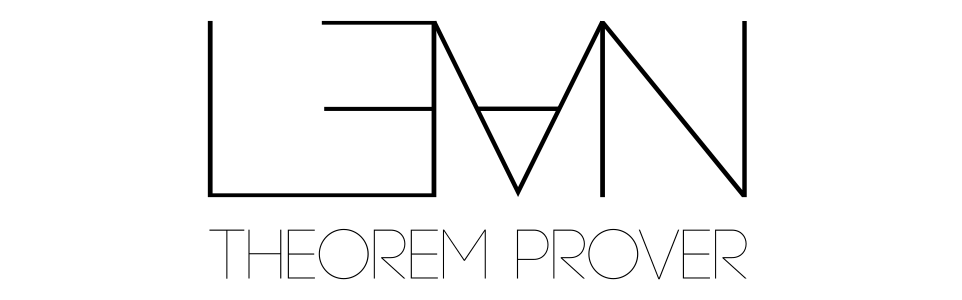
\includegraphics[height=0.8\titleimageht]{logo}
    }
}

\newcommand{\kit}[1]{\textcolor{KITgreen}{#1}}

\begin{document}
\begin{frame}
  \maketitle
\end{frame}

\begin{frame}[fragile,t]{The Lean theorem prover}
  \begin{itemize}
  \item dependently-typed proof assistant
  \item small trusted kernel
  \item also a \kit{purely functional, eager programming language}
  \end{itemize}
  
\begin{leancode}
inductive list (α : Type u)
| nil : list
| cons : α → list → list
\end{leancode}
  \vspace{-0.5cm}
\begin{leancode}
def map (f : α → β) : list α → list β
| []         := []
| (x :: xs') := f x :: map xs'
\end{leancode}

  \begin{center}
    \Large\url{https://leanprover.github.io}
  \end{center}
\end{frame}

\begin{frame}{A brief history of Lean}
  \begin{itemize}
  \item Lean 0.1 (2014)
  \item Lean 2 (2015)
    \begin{itemize}
    \item first official release
    \item fixed tactic language
    \end{itemize}
  \item Lean 3 (2017)
    \begin{itemize}
    \item make Lean a \kit{meta-programming} language: build tactics in Lean
    \item backed by a bytecode interpreter
    \end{itemize}
  \item Lean 4 (201X)
    \begin{itemize}
    \item make Lean a \kit{general-purpose} language: native back end, FFI, ...
    \item reimplement Lean in Lean
    \end{itemize}
  \end{itemize}
\end{frame}

\tikzset{
  invisible/.style={opacity=0},
  visible on/.style={alt={#1{}{invisible}}},
  alt/.code args={<#1>#2#3}{%
    \alt<#1>{\pgfkeysalso{#2}}{\pgfkeysalso{#3}} % \pgfkeysalso doesn't change the path
  },
}

\begin{frame}
\only<1>{\frametitle{Lean 3 backend}}
\only<2>{\frametitle{Lean 4 backend}}
  \begin{center}
    \begin{tikzpicture}[rounded corners, >=stealth, thick, nodes={minimum height=2em}]
      \node[draw] (elab) {elaborator}
        child[->] {
          node[draw] {kernel}
          edge from parent node[left] {term}
        }
        child[->] {
          node[draw] {compiler}
          [sibling distance=3.5cm]
          child[->,visible on=<2>] {
            node[draw] (cpp) {C++ code extraction}
            edge from parent node[right] {IR}
          }
          child[->] {
            node[draw] (interpreter) {interpreter}
            edge from parent node[right] {bytecode}
          }
          child[->, visible on=<2>] {
            node[draw] (llvm) {LLVM backend?}
            edge from parent node[right] {IR}
          }
          edge from parent node[right] {term}
        }
      ;
      \draw[->,dotted] (interpreter) to[out=0,in=0]
        node[right] {tactic execution}
        (elab);
      \uncover<2>{
        \draw[->,dotted] (cpp) to[out=90,in=180] (elab);
        \draw[->,dotted] (llvm) to[out=45,in=0] (elab);
      }
    \end{tikzpicture}
  \end{center} 
\end{frame}

%\begin{frame}{Lean 4 backend}
%  \begin{center}
%    \begin{tikzpicture}[rounded corners, >=stealth, thick, nodes={minimum height=2em}]
%      \node[draw] (elab) {elaborator}
%        child[->] {
%          node[draw] {kernel}
%          edge from parent node[left] {term}
%        }
%        child[->] {
%          node[draw] {compiler}
%          [sibling distance=3.5cm]
%          child[->] {
%            node[draw] (interpreter) {interpreter}
%            edge from parent node[left] {bytecode}
%          }
%          child[->] {
%            node[draw,dotted] {LLVM backend?}
%            edge from parent node[right] {IR}
%          }
%          edge from parent node[right] {term}
%        }
%      ;
%    \end{tikzpicture}
%  \end{center} 
%\end{frame}

\begin{frame}[fragile]{Lean 3 object model}

Uniform model: every value is a \kit{tagged} pointer representing one of
  \begin{itemize}
  \item a 31-bit number
  \item a reference to a ref-counted VM object
    \begin{itemize}
    \item a constructor value
    \item a closure
    \item an arbitrary-precision integer
    \item any C++ object derived from \verb!vm_external!
    \end{itemize}
  \end{itemize}
\end{frame}

\begin{frame}{Lean 3 constructor object}

\begin{description}
\item[4 bytes] reference counter
\item[1 byte\phantom{s}]  object kind
\item[4 bytes] constructor index
\item[4 bytes] \#fields
\item[4/8 bytes] field \#0
\item[...] ...
\end{description} 
\end{frame}

\begin{frame}{Lessons from Lean 3's model}

  \begin{itemize}[<+->]
\item Originally only intended for single-threaded code \\
  $\Longrightarrow$ no need for atomic RC!
\item Eventually needed to move objects between threads \\
  $\Longrightarrow$ fall back to deep-copying...
\item Every object is a C++ smart pointer \\
  $\Longrightarrow$ simple to use, but no way to optimize RC ops
\item Core types like \texttt{name} and \texttt{expr} are not VM objects\\
  $\Longrightarrow$ need to be wrapped in \texttt{vm\_external} for every operation
\end{itemize}

\end{frame}

\begin{frame}{Lean 4 object model}

\kit{Non-uniform} model: in the lowest IR, each value has one of the types
\begin{itemize}
\item \texttt{int8/uint8/.../uint64}: \kit{unboxed} primitive value
\item \texttt{\_obj}: tagged pointer to a VM object
  \begin{itemize}
  \item a constructor, closure, or bigint
  \item \kit{an array of boxed or unboxed values}
  \item \kit{a thunk}
  \end{itemize}
\end{itemize}
\end{frame}

\begin{frame}[fragile]{Lean 4 constructor object}
  
  \begin{description}
  \item[1 byte] object kind
  \item[1 byte] \kit{memory kind}
  \item[2 bytes] constructor index
  \item[2 bytes] \#\kit{boxed} fields
  \item[2 bytes] \#\kit{unboxed bytes}
  \item[4/8 bytes] boxed field \#0
  \item [...] ...
  \item[$X$ bytes] unboxed field \#0
  \item [...] ...
  \end{description}

  All boxed fields come first $\Longrightarrow$ \verb!free! can still be implemented uniformly
\end{frame}

\begin{frame}{Memory kind}
  \begin{itemize}
  \item single-threaded: non-atomic RC
    \begin{itemize}
    \item the default for heap allocations
    \end{itemize}
  \item multi-threaded: atomic RC
    \begin{itemize}
    \item threading primitives \emph{upgrade} object graphs crossing threads to
      this kind
    \item everything is immutable $\Longrightarrow$ ST object never reachable from MT object
    \end{itemize}
  \item stack: no RC
  \item region: no RC
  \end{itemize}
\end{frame}

\begin{frame}{The case for ref counting}
  \begin{itemize}
  \item<+-> writing a good GC is \kit{really hard}
    \begin{quote}
     ``The biggest challenge is implementing the garbage collector.''
    \end{quote}
    \rightline{{\rm -- Multicore OCaml website\footnote{\url{http://ocamllabs.io/doc/multicore.html}}\hspace{1em}}}
  \item<+-> easier to use from other languages
  \item<+-> everything is immutable $\Longrightarrow$ no cycles!
  \item<+-> explicit ref count $\Longrightarrow$ can do destructive updates on $RC=1$
    \begin{itemize}
    \item like linear types, but checked dynamically
      \begin{itemize}
      \item dependent types are hard enough
      \item more precise (but also less predictable)
      \end{itemize}
    \end{itemize}
  \end{itemize}
\end{frame}

\begin{frame}[fragile]{Dynamic linearity}
\vspace{-0.4cm}
\begin{leancode}
def map (f : α → β) : list α → list β
| []         := []
| (x :: xs') := f x :: map xs'
\end{leancode}
\pause
\vspace{-0.7cm}
\begin{leancode}
[compiler.llnf]
λ (f xs : _obj),
  list.cases_on xs
    (let _x_1 : _obj := _dec f
     in _cnstr.0)
    (let _x_1 : _obj := _proj.0 xs,
         _x_2 : _obj := _inc _x_1,
         _x_3 : _obj := _proj.1 xs,
         _x_4 : _obj := _inc _x_3,
         _x_5 : _obj := _reset.2 xs,
         _x_6 : _obj := _apply f _x_2,
         _x_7 : _obj := list.map f _x_4
     in _reuse.1 _x_5 _x_6 _x_7)
\end{leancode}

  \lean{_reset}/\lean{_reuse} check for linearity at runtime\\
  $\Longrightarrow$ unique prefix of a list will be reused even if remainder is shared!
\end{frame}

\begin{frame}[fragile,fragile]{Dynamic linearity}
  Benchmarks of direct C++ implementations of
\begin{leancode}
list.map (+1) (list.range 4000)
\end{leancode}

  \bigskip
  \begin{center}
    \begin{tabular}{l|r}
      optimizations & run time of \lean{map} \\\hline
      no reuse & 214.3 {\mu}s \\
      \lean{_reset}/\lean{_reuse} & 27.7 {\mu}s \\
      optimized reuse & 12.3 {\mu}s \\
      known unique & 10.7 {\mu}s \\
    \end{tabular}
  \end{center}
\end{frame}

\begin{frame}[fragile]{Borrowing}
\vspace{-0.4cm}
\begin{leancode}
def length : @borrowed (list α) → nat
| []         := 0
| (x :: xs') := length xs' + 1
\end{leancode}
\vspace{-0.7cm}
\begin{leancode}
[compiler.llnf]
λ (xs : _obj),
  list.cases_on xs
    0
    (let _x_1 : _obj := _proj.1 xs,
         _x_2 : _obj := length _x_1,
     in nat.add _x_2 1)
\end{leancode}

The \lean{@borrowed} attribute
\begin{itemize}
\item delays/avoids RC operations:
  \begin{itemize}
  \item no inc/dec when passing an argument to a borrow parameter
  \item inc when returning/passing a borrowed value to a non-borrow parameter
  \end{itemize}
\item but prevents linear updates
\end{itemize}
\end{frame}

\begin{frame}[fragile]{Regions: minimizing startup time}
Lean 3 startup does not scale well: deserializing all dependencies can take significant time and memory

\pause
\vfill

Compare with Isabelle: dependencies can be compiled into a single ML heap image
\pause
\begin{itemize}
\item<+-> but at most one heap can be loaded
\item<+-> still needs to be read from disk eagerly
\item<5-> fragile: heaps cannot be created from an IDE session (at the moment)
\end{itemize}

\pause
\vfill

What if we could just \verb!mmap! (multiple!) regions of objects into memory?
\pause
\begin{itemize}
\item<+-> lazy loading and prefetching provided by the OS
  \begin{itemize}
  \item proofs aren't needed usually
  \end{itemize}
\item<+-> everything immutable \\
  $\Longrightarrow$ pages can even be shared by multiple Lean processes
  \begin{itemize}
  \item careful: must not touch RC
  \end{itemize}
\end{itemize}
\end{frame}

\begin{frame}{Regions: minimizing startup time}
We're investigating two approaches:

\bigskip

\kit{Simple approach:} use relative pointers in region objects
\begin{itemize}
\item introduces branch for retrieving unboxed field
%\item TODO: some performance numbers?
\end{itemize}

\pause
\bigskip

  \kit{Advanced approach:} try to \texttt{mmap} each region to its original address
\begin{itemize}
\item on collision: fall back to eager loading and pointer patching
\item probability of a single collision between 100 dependencies of size
  10 MB in 48-bit address space is \textasciitilde0.018\%
\end{itemize}

\pause
\bigskip

In either approach, \emph{writing} objects to disk \kit{does} need some transformations
\end{frame}

\begin{frame}[fragile,fragile]{Regions: minimizing startup time}
  For regions to work, all state to be serialized must be Lean objects

  \pause
  \bigskip

  Unboxed fields now make it feasible to reimplement core types as Lean objects!

%object_ref mk_cnstr(unsigned tag, object_ref const & o1, object_ref const & o2, unsigned scalar_sz = 0) {
%    object * r = alloc_cnstr(tag, 2, scalar_sz);
%    cnstr_set(r, 0, o1.raw()); inc(o1.raw());
%    cnstr_set(r, 1, o2.raw()); inc(o2.raw());
%    return object_ref(r);
%}

\begin{minted}[fontsize=\scriptsize]{c++}
expr mk_const(name const & n, levels const & ls) {
    expr r(mk_cnstr(static_cast<unsigned>(expr_kind::Const), n, ls, expr_scalar_size(expr_kind::Const)));
    set_scalar<expr_kind::Const>(r, hash(n.hash(), hash(ls)), false, has_mvar(ls), false, has_param(ls));
    return r;
}
\end{minted}

  \pause

  Unboxed metadata is at the end of the object\\
  $\Longrightarrow$ can be hidden in the Lean definition

\begin{minted}{lean}
inductive expr
| const : name → list level → expr
| ...
\end{minted}
\end{frame}

\begin{frame}{Implementation status}
  \begin{itemize}
  \item object model runtime in C++
  \item core types ported to model
  \item optimizing compiler from Core Lean to LLNF
    \begin{itemize}
    \item inlining, specialization, simplification
    \item using join-point representation
    \end{itemize}
  \item compiler from LLNF to old bytecode format

    \color{gray}

  \item model used by backends and built-ins
  \item writing and loading regions
  \item multi-threading
  \item borrowing
  \end{itemize}
\end{frame}

\begin{frame}{Conclusion}
  \begin{itemize}
  \item A new object model customized to the needs of a theorem prover
  \item utilizing properties of an eager, purely functional language
  \item designed to avoid allocations during startup and at run time
  \end{itemize}

  \pause
  \vfill

  \begin{center}
    \Huge{Thank you!}
  \end{center}
\end{frame}
\end{document}

%%% Local Variables:
%%% mode: latex
%%% TeX-master: t
%%% TeX-engine: luatex
%%% TeX-command-extra-options: -shell-escape
%%% End:
